\documentclass[12pt]{article}
\usepackage{amsmath}
\usepackage{amssymb}
\usepackage{geometry}
\usepackage{enumerate}
\usepackage{natbib}
\usepackage{float}%稳定图片位置
\usepackage{graphicx}%画图
\usepackage[english]{babel}
\usepackage{a4wide}
\usepackage{indentfirst}%缩进
\usepackage{enumerate}%加序号
\usepackage{multirow}%合并行
\title{\large UM-SJTU JOINT INSTITUTE\\Introduction to Computer Organization\\(VP370)\\\ \\\ \\\ \\\ \\\ \\\ \\\ \\\ \\\ \\\ \\\
 Project 2 Report\\\ \\\ \\\ \\\ \\\ \\\ }
\author{Name: Pan Chongdan\\ID: 516370910121}
\date{Date: \today}

\begin{document}
\maketitle
\newpage
\tableofcontents
\newpage
\section{Introduction and Objective}
Use Vivado and verilog to simulate how MIPS single cycle and pipeline processor works.
\begin{enumerate}[-]
\item The memory-reference instructions load word (lw) and store word (sw).
\item The arithmetic-logical instructions add, addi, sub, and, andi, or, and slt.
\item The jumping instructions branch equal (beq), branch not equal (bne), and jump (j).
\end {enumerate}
\section{Top Level Block Diagram}
\subsection{Single cycle}
\begin{figure}[H]
\centering
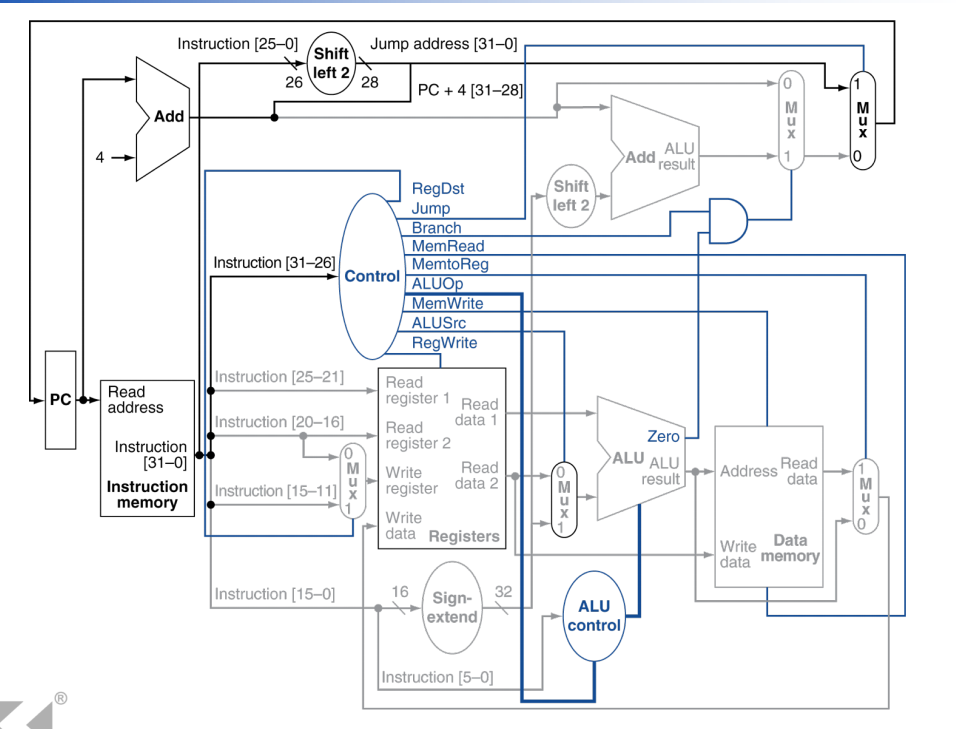
\includegraphics[scale=0.5]{P1.jpg}
\end{figure}

Our design diagram is very similar to the above figure from textbook, but we add a Branch control signal to implement beq and bne.
\subsection{PipeLine}
\section{Design of Components}
\subsection{IF stage}
\subsection{Instruction Memory}
\begin{figure}[H]
\centering
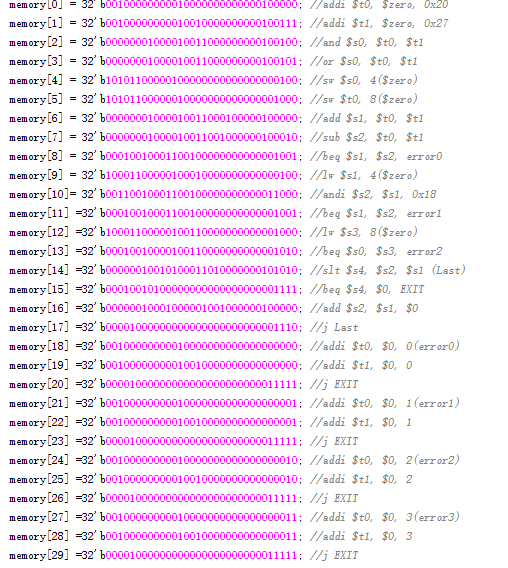
\includegraphics[scale=1]{Instruction.jpg}
\end{figure}
\subsection{ID stage}
\subsection{EX stage}
\subsection{MEM stage}
\subsection{WB stage}
\section{Control and Data Hazard}
\subsection{EX stage}
This part only contain data hazard.
\subsection{ID stage}
\subsubsection{Control Hazard}
\subsubsection{Data Hazard}
\section{Instruction Implementation}
\section{SSD and Top Module}
\subsection{Internal Clock Divider}
\begin{figure}[H]
\centering
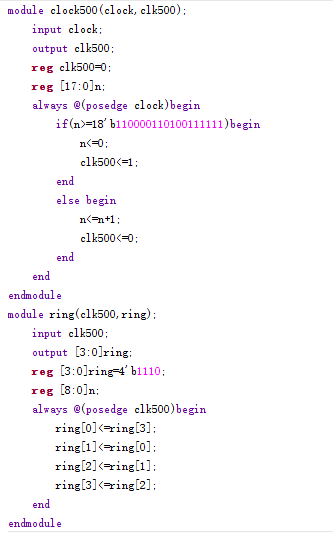
\includegraphics[scale=1]{CD.jpg}
\end{figure}
This module slow down the internal clock of FPGA board to 500 Hz to implement the SSD four digital display.
\subsection{SSD Display}
\begin{figure}[H]
\centering
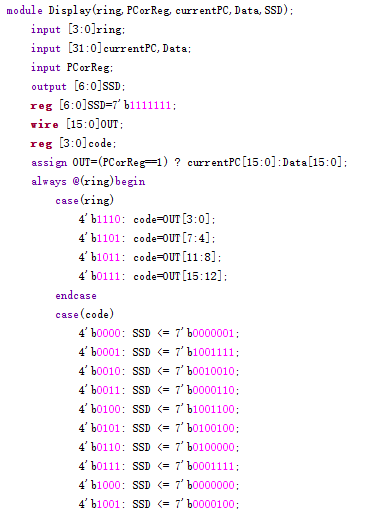
\includegraphics[scale=1]{SSD1.jpg}
\end{figure}
\begin{figure}[H]
\centering
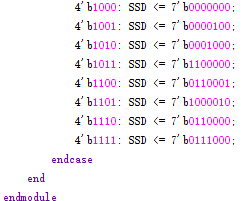
\includegraphics[scale=1]{SSD2.jpg}
\end{figure}
This module directly control the SSD hexadecimal display, including selection for PC value and register value.
\subsection{Constrain File}
The constrain file shows the connection of the port and signal.
\begin{figure}[H]
\centering
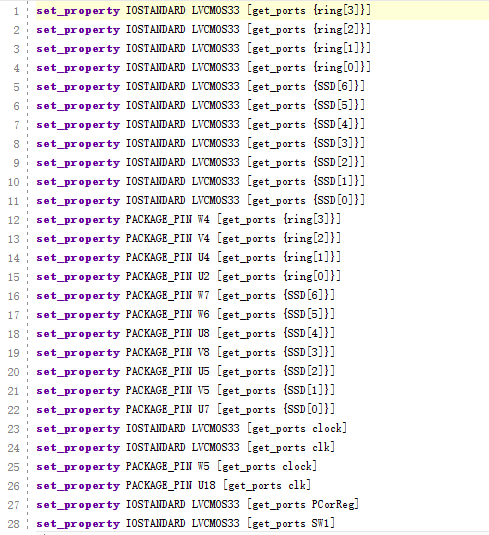
\includegraphics[scale=1]{xdc1.jpg}
\end{figure}
\begin{figure}[H]
\centering
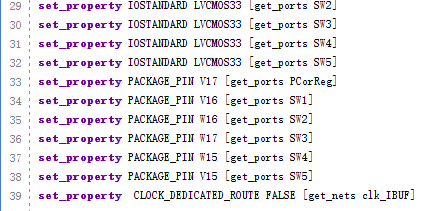
\includegraphics[scale=1]{xdc2.jpg}
\end{figure}
\section{Textual Result}
By running the instruction memory, we can achieve Textual Result which is contained in Appendix. 
\section{Conclusion and Discussion}
\subsection{Single Cycle}
For single cycle part, the project asks us to implement both beq and bnq instructions, which is different from Slies. As a result, we increase one bit to ALUop and add a signal. Since the MIPS processor must implement much more instruction in reality, the ALUop must have more bits and the controller will generate more signals.
\section{Reference}
\begin{enumerate}[-]
\item VE370 Course. Description of Project 4.
\item Zheng Gang L6 Single Cycle Processor
\item Zheng Gang L7 Pipeline Processor
\item Zheng Gang L8 Data Hazard
\item Zheng Gang L9 Control Hazard
\end{enumerate}
\section{Appendix}
\subsection{Single Cycle Textual Result}
\begin{figure}[H]
\centering
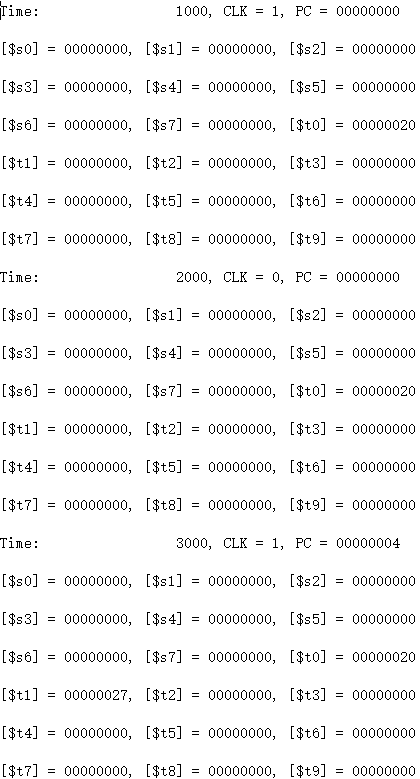
\includegraphics[scale=1]{R1.jpg}
\end{figure}
\begin{figure}[H]
\centering
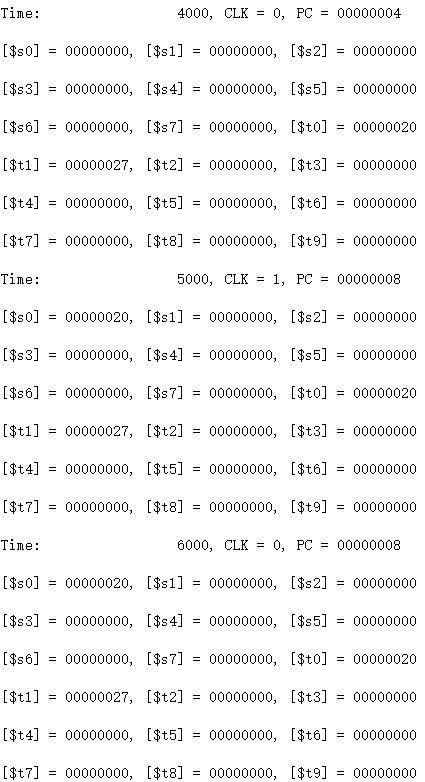
\includegraphics[scale=1]{R2.jpg}
\end{figure}
\begin{figure}[H]
\centering
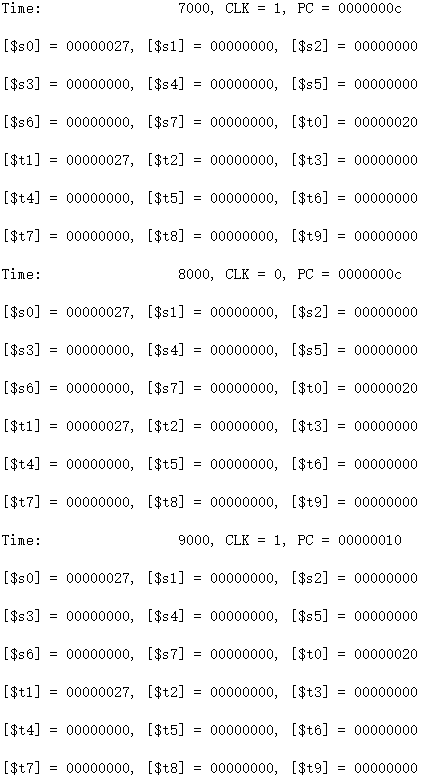
\includegraphics[scale=1]{R3.jpg}
\end{figure}
\begin{figure}[H]
\centering
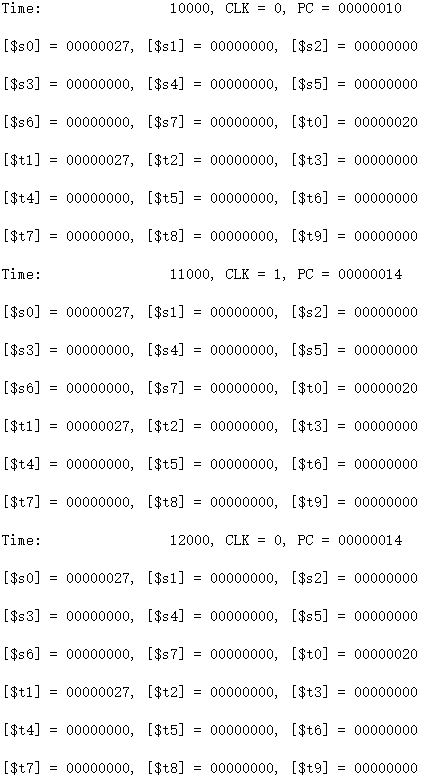
\includegraphics[scale=1]{R4.jpg}
\end{figure}
\begin{figure}[H]
\centering
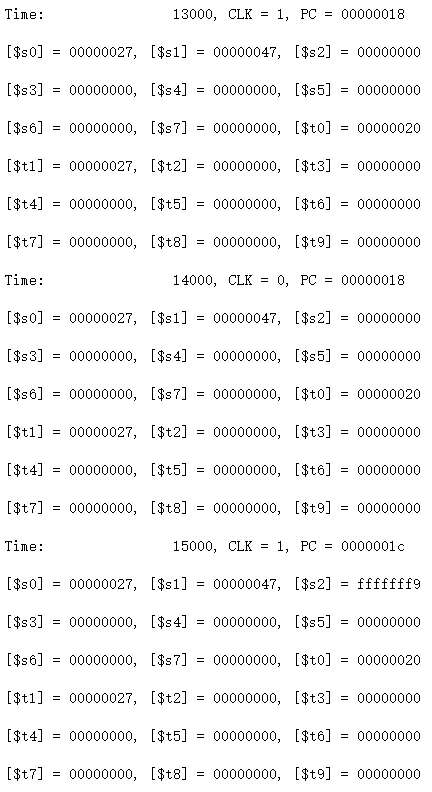
\includegraphics[scale=1]{R5.jpg}
\end{figure}
\begin{figure}[H]
\centering
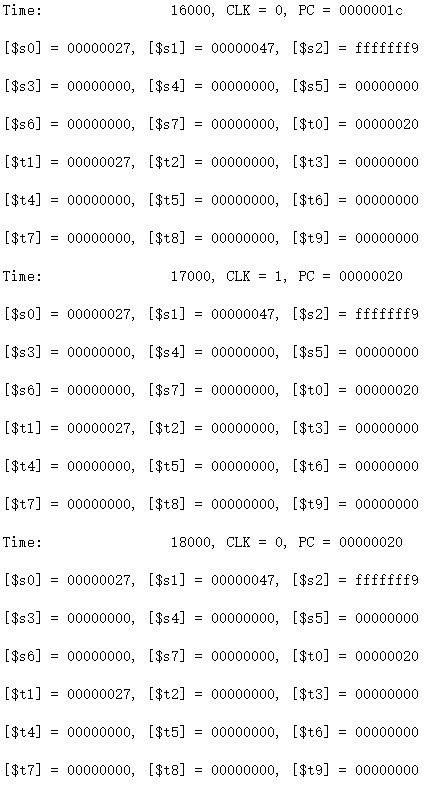
\includegraphics[scale=1]{R6.jpg}
\end{figure}
\begin{figure}[H]
\centering
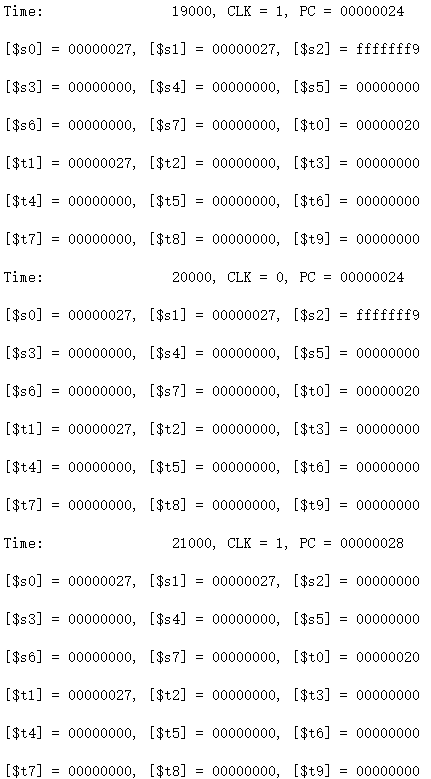
\includegraphics[scale=1]{R7.jpg}
\end{figure}
\begin{figure}[H]
\centering
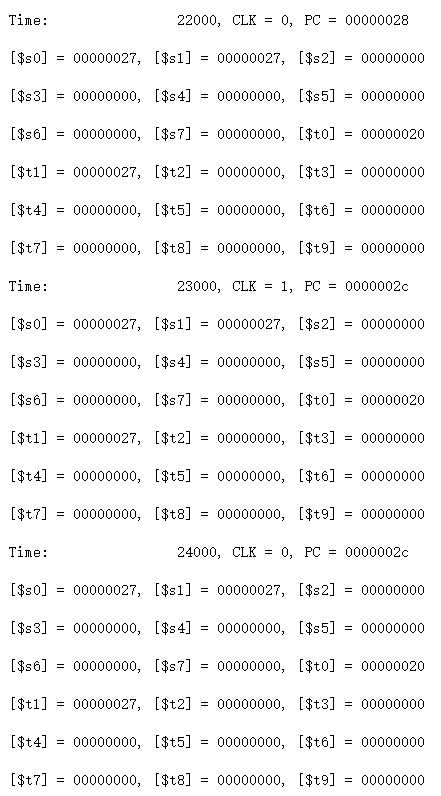
\includegraphics[scale=1]{R8.jpg}
\end{figure}
\begin{figure}[H]
\centering
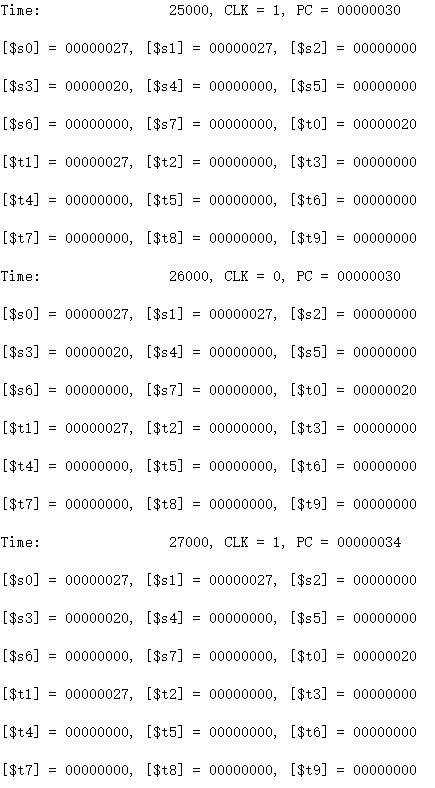
\includegraphics[scale=1]{R9.jpg}
\end{figure}
\begin{figure}[H]
\centering
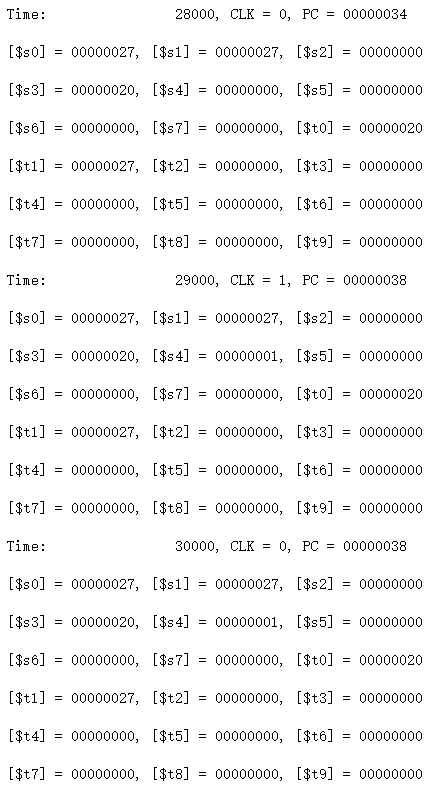
\includegraphics[scale=1]{R10.jpg}
\end{figure}
\begin{figure}[H]
\centering
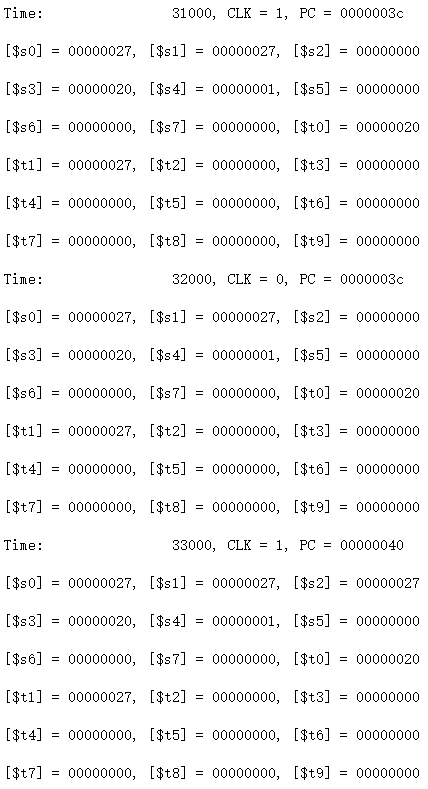
\includegraphics[scale=1]{R11.jpg}
\end{figure}
\begin{figure}[H]
\centering
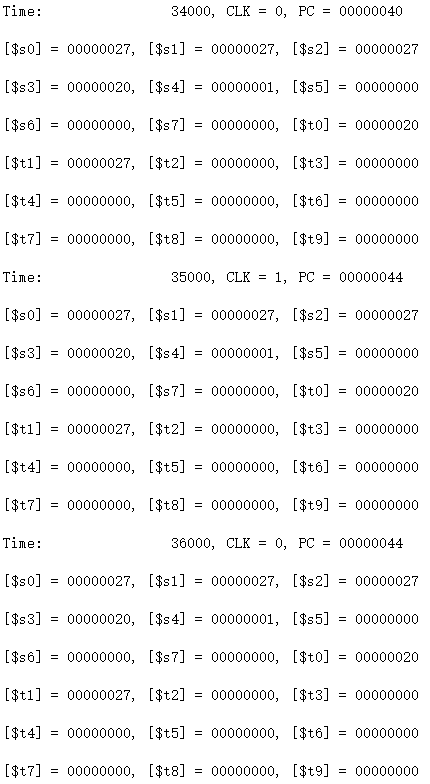
\includegraphics[scale=1]{R12.jpg}
\end{figure}
\begin{figure}[H]
\centering
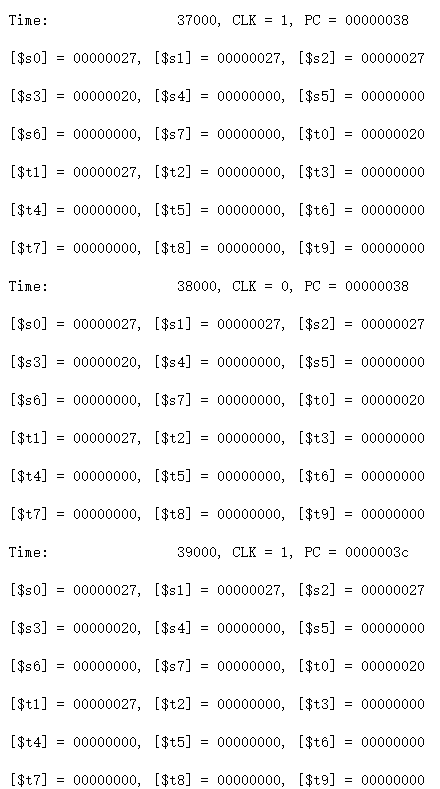
\includegraphics[scale=1]{R13.jpg}
\end{figure}
\begin{figure}[H]
\centering
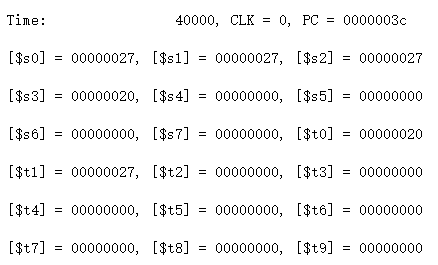
\includegraphics[scale=1]{R14.jpg}
\end{figure}
\end{document}